\noindent \justifying

\section{Previo}

\subsection{Identificar un sistema dinámico que se tenga en casa y definir la salida y la entrada del mismo (para discusión en clase)}

Un sistema dinámico es un sistema complejo que presenta un cambio o evolución de su estado en un tiempo, el comportamiento en dicho estado se puede caracterizar determinando los límites del sistema, los elementos y sus relaciones; de esta forma se puede elaborar modelos que buscan representar la estructura del mismo sistema.\\
Un ejemplo de un sistema dinámico se puede ver en una especie de peces que se reproduce de tal forma que este año la cantidad de peces es Xk, el año próximo será Xk + 1. De esta manera podemos poner nombres a las cantidades de peces que habrá cada año, así: año inicial X0, año primero X1,..., año k Xk.\\
Entrada:Viejos peces (padres).\\
Salida:Nuevos peces (hijos).\\	
Como se puede observar, se cumple para cualquier año k; lo cual significa que la cantidad de peces se puede determinar si se sabe la cantidad del año anterior. Por consiguiente esta ecuación representa un sistema dinámico, o el clima también puede ser un ejemplo.\\


La respuesta a esta pregunta servirá para responder la pregunta a la siguiente, ya que si pensamos en un sistmea de orden mayor a partir de un ejemplo podríamos determinar como funcionaría para para uno de orden mayor, en este caso encontré un ejemplo especificado de orden mayor de algo que se encuentra en nuestras casas como es la bomba del agua (se encuentra en el Tinaco)



\subsection{¿Como analizaría un sistema de orden mayor?}

Para analizar un sistema de orden superior empezamos por escribir su función de transferencia:
\begin{equation}
	H(s)=K\frac{(s-z_1)(s-z_2)...(s-z_n)}{(s-p_1)(s-p_2)(s-p_n)}
\end{equation} 
La mayor parte de la información de como funciona el ssitema nos la darán la localización de los polos y ceros. Esto determina si el sistema es estable o no.\\
En caso de tener polos reales la ecuación toma la siguiente forma:
\begin{equation}
	H(s)=\frac{a_1}{s-p_1}+...+\frac{a_n}{s-p_n}
\end{equation}
A partir de aquí analizamos su respuesta a un impulso y un escalón, quedándonos sus ecuaciones de una de las siguientes formas respectivamente:
\begin{equation}
	y_{imp}=\alpha_1 e^{p_1t}+..+\alpha_n e^{p_nt}
\end{equation}
\begin{equation}
	y_{step}=\beta_0 + \beta_1 e^{p_1t}+...+ \beta_n e^{p_nt}
\end{equation}
Cada polo real p genera un término exponencial en la respuesta. El comportamiento de las oscilaciones va a depender de si la parte real del poplo es negativa o positiva, mientras que la magnitud depende de los ceros.\\
En el caso de un sistema de segundo orden podemos escribir su ecuación característica en términos de zeta y omega, de la siguiente forma:
\begin{equation}
	\frac{d^2y(t)}{dt^2}+2\zeta \omega_n \frac{dy(t)}{dt}+(\omega_n)^2y(t)=k(\omega_n)^2x(t)
\end{equation}
A partir de su respuesta en la ecuación homogénea podemos llegar a un polinimio de la siguiente forma:
\begin{equation}
	s^2+2\zeta\omega_ns+\omega^2_n=0
\end{equation}
La respuesta del sistema va a depender de los valores que tenga el término $\zeta$, siendo sus valores posibles entre cero e infinito positivo. Lo que nos interesará para el diseño de un sistema es que su valor sea mayor o igual a uno.



\textbf{Ejemplo:}

Tengo que decir que la manera de analizarlo y de resolverlo en este caso no son la misma, ya que existen varios métodos, aunque tienen cosas en común.

\begin{figure}[H]
	\centering
	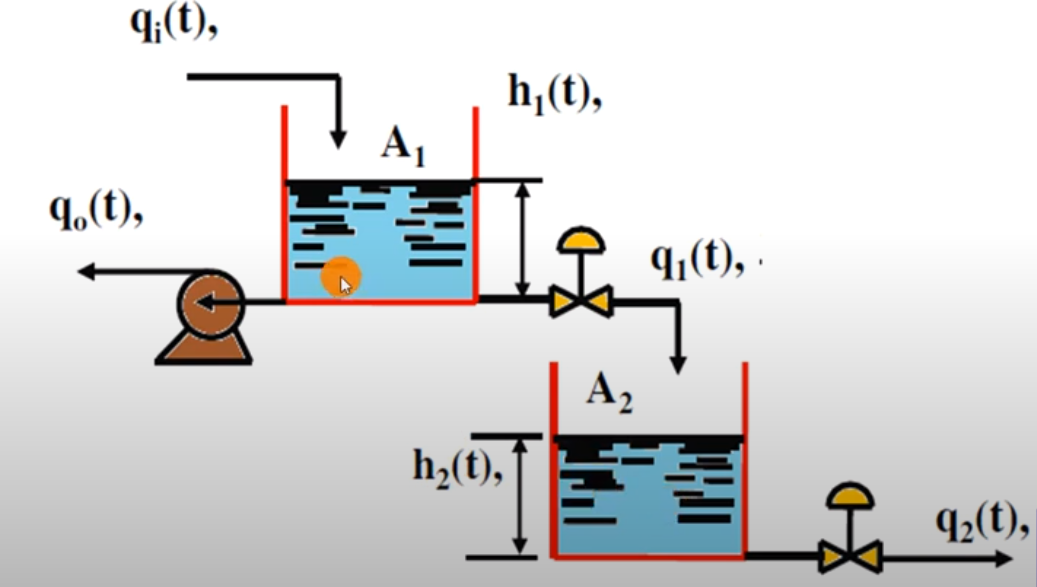
\includegraphics[width=0.7\linewidth]{img/s3}
	\caption{Tanques en serie}
	\label{fig:s3}
\end{figure}


En este caso será un sistema dinámico de orden superior, pero que además es no interactivo ya que el flujo del recipiente A2 no interfiere el de A1, pero A2 si depende del flujo de A1.

$$ A1 \frac{dh_1}{dt} = q_i-q_1-q_0 $$
$$\frac{dht}{dt}=0$$
$$q_1=k_1 \sqrt{h_1} $$
$$q_0=k_0 \sqrt{h_1} $$
$$q_0= \Delta (dA_v) \sqrt{2 \zeta h_1}  $$
$$A_1 \frac{dh_1}{df}=q_i-(k_1 +k_0) \sqrt{h_1} $$
$$p.o \rightarrow q_{io} $$
$$h_o=\frac{q_{io}}{k_1 +k_0}  $$
$$\frac{A_1 dh_1(t)}{dt}=q_i - \frac{t_1 + k_0}{2\sqrt{h_{10}}} $$
$$\frac{A_1 dh_1(t)}{dt} +\frac{t_1 + k_0}{2\sqrt{h_{10}}} =q_i $$
$$\frac{2 \sqrt{h_{10} \cdot A_1}}{k_1 + k_0} \cdot \frac{dh_1}{dt} + h_1 = frac{2 \sqrt{h_{10} \cdot A_1}}{k_1 + k_0} \cdot q_i$$
$$\tau_1 sh_1 + h_1=k_{p1} \cdot q_i $$
$$h_1 = \frac{h_1=k_{p1} \cdot q_i}{\tau_1 sh_1}$$

Ahora vamos a analizar el tanque $ A_2 $

$$A_2 \frac{dh_2}{dt}=q_1 - q_2 $$
$$A_2 \frac{dh_2}{dt}= k_| \sqrt{h_1} - k_2 \sqrt{h_2}$$

En estado estable

$$\frac{dh_2}{dt}=0 \Rightarrow K_1 \sqrt{h_1} =k_2 \sqrt{h_2} $$
$$h_{20} = (\frac{k_1}{k_2})^{2} \cdot h_{10} $$
$$
\frac{A_{2} \partial h_{2}(t)}{\partial t}=\frac{\hbar_{1}}{2 \sqrt{h_{1}}} \cdot h_{1}-\frac{k_{2}}{\partial \sqrt{h_{2} 0}} \cdot h_{2}
$$
$$
A_{2} S h_{2}=\frac{\hbar_{1}}{2 \sqrt{h_{1} 0}} \cdot h_{1}-\frac{k_{2}}{2 \sqrt{h_{2}}} \cdot h_{2}
$$
$$
A_{2} S h_{2}=\frac{K_{1}}{2 \sqrt{h_{1} 0}} \cdot \frac{\hbar_{p_{1}} q_{i}}{\left(N_{1} s+1\right)}-\frac{k_{2} h_{2}}{\sqrt{n_{2} 0}}
$$
$$\frac{A_2 \cdot 2 \sqrt{h_{20}}}{k_2} \cdot Sh_1 + h_2 = \sqrt{\frac{h_{20}}{h_{10}}} \cdot \frac{k_1 k_{p1} q_i}{k_2 (\tau_1 s +1)} $$
$$
\tau_{2} s h_{2}+h_{2}=\frac{K_{P_{2}} q_{i}}{\tau_{1} s+1}
$$
$$h_2= \frac{K_{p2} \cdot q_i}{(\tau_2 s +1) (\tau_1 s +1)}$$

En este caso debido a la la dependecia y a que un factor tiene más peso que otro, el modelo puede simplificarse como

\begin{equation}
	h_{2}(s)=\frac{k_{p_{2}} q_{i}}{\left(\tau_{1} s+1\right)} e^{t / \tau_{.}}
\end{equation} 

\subsection{¿Cuál es la importancia de la constante de tiempo $\tau$ y el factor de amortiguamiento $\zeta$ ?}

\textbf{Constante de tiempo $ \tau $:}

''La constante de tiempo de un sistema de primer orden, generalmente denotada por la letra griega $ \tau $ (tau), se define como el tiempo requerido para que el sistema alcance el 63,2\% del valor final o de estado estable. Por lo tanto la constante muestra la velocidad del sistema ante una determinada entrada para alcanzar el regimen permanente.

Cuanto menor es la constante de tiempo, más rápida es la respuesta del sistema. Si la constante de tiempo es mayor, el sistema se mueve lentamente en su respuesta transitoria.

Entonces, la respuesta transitoria se define como la dinámica del sistema desde el estado inicial hasta alcanzar el estado estacionario, donde en un sistema de primer orden la respuesta transitoria tiene una duración de 4 veces la constante de tiempo''


\textbf{Constante \textbf{$\zeta$}:}

Es aquella que sirver como paramétro para saber que tan rapido se estabilizará un sistemas y llegará a su estado final, si es uno se dice que es un amortiguamiento crítico y es aquel que no pasa el estado de reposo y que además se estabiliza lo antes posible , veamos que esta constante te puede decir como se comportará el sistema en caso de ser estable.


\begin{figure}[H]
	\centering
	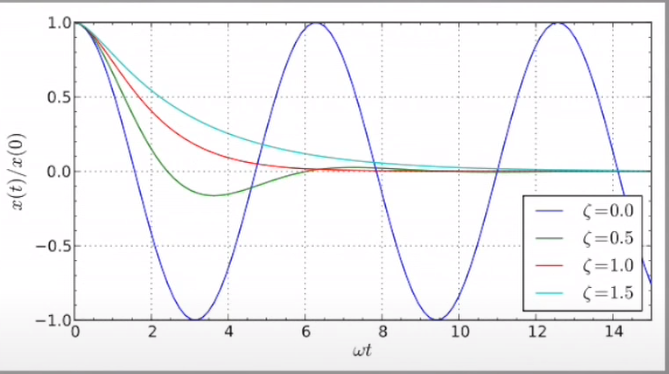
\includegraphics[width=0.7\linewidth]{img/S1}
	\caption{Gráfico que muestra la constante $\zeta$}
	\label{fig:s1}
\end{figure}


Esta mejor explicado en el siguiente video

\url{https://www.youtube.com/watch?v=mD2OKGiwebA}

